\chapter{}
\label{lecture1}
Мы начинаем первую часть нашего курса. Эта часть --- <<Вариационное исчисление>>.
\section{Определение функционала. Примеры вариационных задач.}
\label{lecture1section1}
До сих пор вам в основном встречалось два типа зависимостей:
\begin{enumerate}
	\item Функция: каждому числу или совокупности чисел (в случае функции многих переменных) ставится в соответствие число или совокупность чисел (в случае вектор-функции).
	
	\item Оператор: каждой функции или набору функций ставится в соответствии функция или набор функций. Например, если рассматривать оператор дифференцирования на функциях имеющих производную, то $f(x)\to f'(x)$, или $f(x_1,\ldots,x_n)\?\to f(\phi_1(x_1),\ldots,\phi_n(x_n))$, где $\phi_i(x_i)$ --- некоторые функции.
	
\end{enumerate}

Вариационное исчисление изучает другие зависимости --- когда каждой функции или набору функций из определённого класса ставится в соответствие число.\\
Примеры:
\begin{enumerate1}
	\item $S[f]=\int\limits_a^b f(x)\,\dd{x}$ --- площадь заштрихованной фигуры, $f(x)\in \Cfn[{[a,b]}]{}$.
	\begin{figure}[H]\centering
	\tikzset{every picture/.style={line width=0.75pt}} %set default line width to 0.75pt        
	
	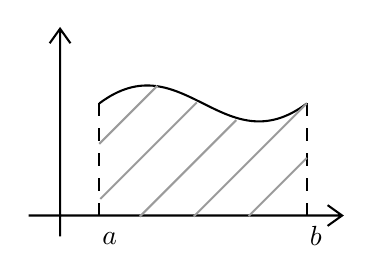
\begin{tikzpicture}[x=0.75pt,y=0.75pt,yscale=-1,xscale=1]
		%uncomment if require: \path (0,142); %set diagram left start at 0, and has height of 142
		
		%Shape: Axis 2D [id:dp819600743870198] 
		\draw  (57,105) -- (208,105)(72.1,15) -- (72.1,115) (201,100) -- (208,105) -- (201,110) (67.1,22) -- (72.1,15) -- (77.1,22)  ;
		%Curve Lines [id:da06782546481569751] 
		\draw    (91,51) .. controls (131,21) and (151,81) .. (191,51) ;
		%Straight Lines [id:da30279113153735726] 
		\draw  [dash pattern={on 4.5pt off 4.5pt}]  (91,51) -- (91,105.5) ;
		%Straight Lines [id:da6946884097796024] 
		\draw  [dash pattern={on 4.5pt off 4.5pt}]  (191,51) -- (191,105.5) ;
		%Straight Lines [id:da08980597198305262] 
		\draw [color={rgb, 255:red, 155; green, 155; blue, 155 }  ,draw opacity=1 ]   (191,77.25) -- (163,105.25) ;
		%Straight Lines [id:da18207740263127015] 
		\draw [color={rgb, 255:red, 155; green, 155; blue, 155 }  ,draw opacity=1 ]   (191,51) -- (136.5,105.5) ;
		%Straight Lines [id:da7156119647134078] 
		\draw [color={rgb, 255:red, 155; green, 155; blue, 155 }  ,draw opacity=1 ]   (157,59) -- (110.5,105.5) ;
		%Straight Lines [id:da5864249578728782] 
		\draw [color={rgb, 255:red, 155; green, 155; blue, 155 }  ,draw opacity=1 ]   (138,50.5) -- (91.5,97) ;
		%Straight Lines [id:da25902283366089773] 
		\draw [color={rgb, 255:red, 155; green, 155; blue, 155 }  ,draw opacity=1 ]   (119,42.5) -- (91,70.5) ;
		
		% Text Node
		\draw (91,111.9) node [anchor=north west][inner sep=0.75pt]    {$a$};
		% Text Node
		\draw (191,108.9) node [anchor=north west][inner sep=0.75pt]    {$b$};
		
		
	\end{tikzpicture}
	\caption{~}
	\label{l1:fig:1}
	\end{figure}
	\item $l[f]=\int\limits_a^b\sqrt{1+f^{\prime 2}(x)}\,\dd{x}$ --- длина кривой, $f\in \Cfn[{[a,b]}]{1}$ --- класс непрерывно дифференцируемых на ${[a,b]}$ функций.
\end{enumerate1}

\noindent Дадим общее определение для подобного рода зависимостей.
\begin{Def}
	Пусть $\mc{K}=\{f(x_1,\ldots,x_n)\}$ --- класс каких-то функций $f(x_1,\ldots,x_n)$, определённых в области $\mc{D}$ $n$-мерного пространства. Будем говорить, что \textbf{задан функционал $\pmb{\J[f]}$}, если задан закон, по которому каждой функции $f\in\mc{K}$ ставится в соответствие число $\J[f]$. Это число обозначается $\J[f]$ и называется значением функционала на функции $f$.
\end{Def}

\noindent В приведённых выше примерах \\
\indent$S[f]$ задан на $\mc{K}=\big\{f(x)\big|f\in \Cfn[{[a,b]}]{}\big\}$,\\
\indent $l[f]$ задан на $\mc{K}=\big\{f(x)\big|f\in \Cfn[{[a,b]}]{1}\big\}$.\\
Разумеется, могут быть и другие классы для функционалов $S[f]$ и $l[f]$ в зависимости от рассматриваемых задач.

Исследуя свойства функций в курсе математики, вы решали задачи о нахождении экстремумов функций, однако целый ряд задач требует отыскания экстремумов не функций, а функционалов. Именно этим и занимается <<Вариационное исчисление>>.
\vspace{0.25cm}

Приведём примеры задач, решаемых в вариационном исчислении.
\newlist{enumerate2}{enumerate}{1}
\setlist[enumerate2,1]{label=\arabic*., ref=\arabic*.} 

\begin{enumerate2}
	\item \textbf{Задача о кривой наискорейшего спуска (задача о брахистохроне)}.\\
	Пусть на вертикальной плоскости $x,y$ заданы две точки $A(a, y_0)$ и $B(b, y_1)$, $y_1<y_0$.
	
	\begin{figure}[H]\centering
	\tikzset{every picture/.style={line width=0.75pt}} %set default line width to 0.75pt        
	
	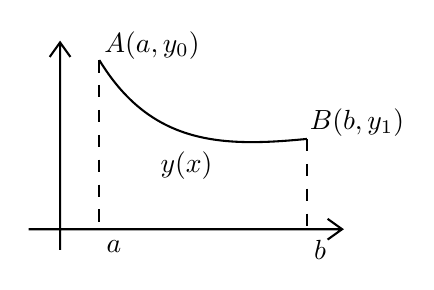
\begin{tikzpicture}[x=0.75pt,y=0.75pt,yscale=-1,xscale=1]
		%uncomment if require: \path (0,142); %set diagram left start at 0, and has height of 142
		
		%Shape: Axis 2D [id:dp5296256236644323] 
		\draw  (57,105) -- (208,105)(72.1,15) -- (72.1,115) (201,100) -- (208,105) -- (201,110) (67.1,22) -- (72.1,15) -- (77.1,22)  ;
		%Curve Lines [id:da5139961929878707] 
		\draw    (91,23.5) .. controls (116,64.5) and (150,65.5) .. (191,61.5) ;
		%Straight Lines [id:da7749819981896289] 
		\draw  [dash pattern={on 4.5pt off 4.5pt}]  (91,23.5) -- (91,105.5) ;
		%Straight Lines [id:da17627525123267485] 
		\draw  [dash pattern={on 4.5pt off 4.5pt}]  (191,61.5) -- (191,105.5) ;
		
		% Text Node
		\draw (93,108.9) node [anchor=north west][inner sep=0.75pt]    {$a$};
		% Text Node
		\draw (193,108.9) node [anchor=north west][inner sep=0.75pt]    {$b$};
		% Text Node
		\draw (92,8.4) node [anchor=north west][inner sep=0.75pt]    {$A( a,y_{0})$};
		% Text Node
		\draw (191,45.4) node [anchor=north west][inner sep=0.75pt]    {$B( b,y_{1})$};
		% Text Node
		\draw (119,66.4) node [anchor=north west][inner sep=0.75pt]    {$y( x)$};
		
		
	\end{tikzpicture}
	\caption{~}
	\label{l1:fig:2}
	\end{figure}
	Задача: найти кривую, соединяющую точки $A$ и $B$, по которой материальная точка скатится из $A$ в $B$ за минимальное время.
	
	Пусть $y(x)$ --- произвольная допустимая кривая. Найдём время скатывания по этой кривой. Разобъём отрезок ${[a,b]}$ на $n$ частей 
	\begin{equation*}
		\Delta x\eqdef\dfrac{b-a}{n}
	\end{equation*} 
	и определим время скатывания по элементарному отрезку кривой над $\Delta x$.
	\begin{figure}[H]\centering
	\tikzset{every picture/.style={line width=0.75pt}} %set default line width to 0.75pt        
	
	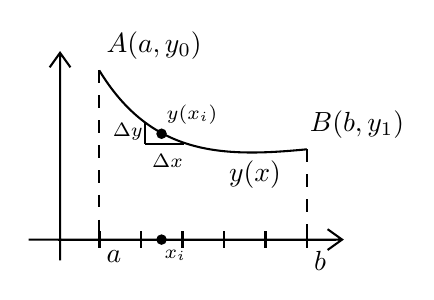
\begin{tikzpicture}[x=0.75pt,y=0.75pt,yscale=-1,xscale=1]
		%uncomment if require: \path (0,142); %set diagram left start at 0, and has height of 142
		
		%Shape: Axis 2D [id:dp3120006234200525] 
		\draw  (57,105) -- (208,105)(72.1,15) -- (72.1,115) (201,100) -- (208,105) -- (201,110) (67.1,22) -- (72.1,15) -- (77.1,22)  ;
		%Curve Lines [id:da5633806752426602] 
		\draw    (91,23.5) .. controls (116,64.5) and (150,65.5) .. (191,61.5) ;
		%Straight Lines [id:da19712351894158475] 
		\draw  [dash pattern={on 4.5pt off 4.5pt}]  (91,23.5) -- (91,105.5) ;
		%Straight Lines [id:da4773530776083561] 
		\draw  [dash pattern={on 4.5pt off 4.5pt}]  (191,61.5) -- (191,105.5) ;
		%Straight Lines [id:da5754475621627722] 
		\draw    (71.1,105) -- (205,105) (91.1,101) -- (91.1,109)(111.1,101) -- (111.1,109)(131.1,101) -- (131.1,109)(151.1,101) -- (151.1,109)(171.1,101) -- (171.1,109)(191.1,101) -- (191.1,109) ;
		%Straight Lines [id:da416850289861296] 
		\draw    (113,59) -- (132.05,59) ;
		%Straight Lines [id:da9627818333382503] 
		\draw    (113,48.5) -- (113,59) ;
		%Flowchart: Connector [id:dp8284141548912727] 
		\draw  [fill={rgb, 255:red, 0; green, 0; blue, 0 }  ,fill opacity=1 ] (119,105) .. controls (119,103.9) and (119.9,103) .. (121,103) .. controls (122.1,103) and (123,103.9) .. (123,105) .. controls (123,106.1) and (122.1,107) .. (121,107) .. controls (119.9,107) and (119,106.1) .. (119,105) -- cycle ;
		%Flowchart: Connector [id:dp5793213628332867] 
		\draw  [fill={rgb, 255:red, 0; green, 0; blue, 0 }  ,fill opacity=1 ] (119,54) .. controls (119,52.9) and (119.9,52) .. (121,52) .. controls (122.1,52) and (123,52.9) .. (123,54) .. controls (123,55.1) and (122.1,56) .. (121,56) .. controls (119.9,56) and (119,55.1) .. (119,54) -- cycle ;
		
		% Text Node
		\draw (93,108.9) node [anchor=north west][inner sep=0.75pt]    {$a$};
		% Text Node
		\draw (193,108.9) node [anchor=north west][inner sep=0.75pt]    {$b$};
		% Text Node
		\draw (93,3.4) node [anchor=north west][inner sep=0.75pt]    {$A( a,y_{0})$};
		% Text Node
		\draw (191,41.4) node [anchor=north west][inner sep=0.75pt]    {$B( b,y_{1})$};
		% Text Node
		\draw (152,65.4) node [anchor=north west][inner sep=0.75pt]    {$y( x)$};
		% Text Node
		\draw (115,62.4) node [anchor=north west][inner sep=0.75pt]  [font=\scriptsize]  {$\Delta x$};
		% Text Node
		\draw (96,47.4) node [anchor=north west][inner sep=0.75pt]  [font=\scriptsize]  {$\Delta y$};
		% Text Node
		\draw (121,108.4) node [anchor=north west][inner sep=0.75pt]  [font=\scriptsize]  {$x_{i}$};
		% Text Node
		\draw (122,38.4) node [anchor=north west][inner sep=0.75pt]  [font=\scriptsize]  {$y( x_{i})$};
		
		
	\end{tikzpicture}
	\caption{~}
	\label{l1:fig:3}
	\end{figure}
	Длина этого участка
	\begin{equation*}
		\sqrt{(\Delta x)^2+(\Delta y)^2}=\sqrt{1+\left(\frac{\Delta y}{\Delta x}\right)^2}\cdot \Delta x.
	\end{equation*}
	Пусть $v(x_i, y_i)$ --- скорость на участке $\Delta x$. Тогда элементарное время скатывания
	\begin{equation*}
		\Delta t= \displaystyle \frac{\sqrt{1+\left(\frac{\Delta y}{\Delta x}\right)^2}\cdot \Delta x}{v(x_i, y_i)}. 
	\end{equation*}
	Суммируя по всем элементарным участкам $\Delta x$ и переходя к пределу при $n\to\infty$, получим время скатывания по кривой $y(x)$.
	\begin{equation*}
		 T[y]=\int\limits_a^b\frac{\sqrt{1+y^{\prime 2}}}{v(x,y)}\,\dd{x}.
	\end{equation*}
	Величину скорости находим из закона сохранения энергии. Пусть $m$ --- масса материальной точки, начальная скорость скатывания равна 0; тогда при $x=a$ потенциальная энергия равна $m\cdot g\cdot y_0$, кинетическая равна нулю. В точке $x$ потенциальная энергия равна $m\cdot g\cdot y$, а кинетическая --- $\frac{m\cdot v^2}{2}$. Таким образом
	\begin{equation*}
		m\cdot g\cdot y_0=m\cdot g\cdot y+\frac{m\cdot v^2}{2}\quad\Rightarrow \quad v=\sqrt{2\cdot g\cdot(y_0-y)}.
	\end{equation*}
	Таким образом  
	\begin{equation*}
		 T[y]=\int\limits_a^b\frac{\sqrt{1+y^{\prime 2}}}{\sqrt{2\cdot g\cdot(y_0-y)}}\,\dd{x}.
	\end{equation*}
	
	Класс $\mc{K}$ допустимых кривых $y=y(x)$ в этой задаче описывается равенством 	
	\begin{equation*}
		\mc{K}=\big\{y(x)\big|y\in\Cfn[{[a,b]}]{1}, y(a)=y_0, y(b)=y_1\big\}.
	\end{equation*}
	Таким образом надо найти $\min\limits_{y\in\mc{K}}\,T[y]$. Функция, дающая минимум (или максимум) функционала, называется \emph{минимайзером} (или \emph{максимайзером}). Минимайзер рассматриваемой задачи --- кривая наискорейшего спуска. Она называется брахистохрона.
	
	\item \textbf{Задача о геодезических.}\\
	Пусть в пространстве $\mathbb{R}^3$ задана поверхность $\phi(x,y,z)=0$ и $A(a_0,b_0,c_0)$, $B(a_1,b_1,c_1)$ --- произвольные точки на поверхности.
	
	\begin{figure}[H]\centering
	\tikzset{every picture/.style={line width=0.75pt}} %set default line width to 0.75pt        
	
	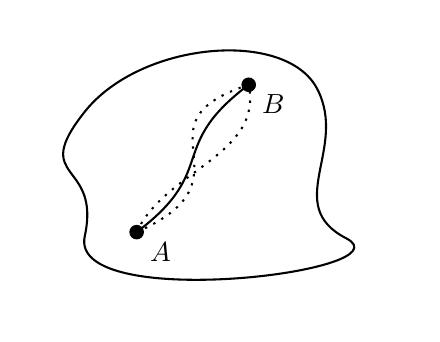
\begin{tikzpicture}[x=0.75pt,y=0.75pt,yscale=-1,xscale=1]
		%uncomment if require: \path (0,124); %set diagram left start at 0, and has height of 124
		
		%Shape: Polygon Curved [id:ds7004080197938745] 
		\draw   (92,35) .. controls (119,1) and (189,-5) .. (204,24) .. controls (219,53) and (187,80) .. (218,96) .. controls (249,112) and (84,132) .. (92,95) .. controls (100,58) and (65,69) .. (92,35) -- cycle ;
		%Flowchart: Connector [id:dp6316722605629903] 
		\draw  [fill={rgb, 255:red, 0; green, 0; blue, 0 }  ,fill opacity=1 ] (114,93) .. controls (114,91.34) and (115.34,90) .. (117,90) .. controls (118.66,90) and (120,91.34) .. (120,93) .. controls (120,94.66) and (118.66,96) .. (117,96) .. controls (115.34,96) and (114,94.66) .. (114,93) -- cycle ;
		%Flowchart: Connector [id:dp17981276820818448] 
		\draw  [fill={rgb, 255:red, 0; green, 0; blue, 0 }  ,fill opacity=1 ] (168,22) .. controls (168,20.34) and (169.34,19) .. (171,19) .. controls (172.66,19) and (174,20.34) .. (174,22) .. controls (174,23.66) and (172.66,25) .. (171,25) .. controls (169.34,25) and (168,23.66) .. (168,22) -- cycle ;
		%Curve Lines [id:da15915648969896234] 
		\draw    (117,93) .. controls (157,63) and (131,52) .. (171,22) ;
		%Curve Lines [id:da7096853264238667] 
		\draw  [dash pattern={on 0.84pt off 2.51pt}]  (117,93) .. controls (176,67) and (113,41) .. (171,22) ;
		%Curve Lines [id:da6619831022453118] 
		\draw  [dash pattern={on 0.84pt off 2.51pt}]  (117,93) .. controls (131,63) and (178,56) .. (171,22) ;
		
		% Text Node
		\draw (122,96.4) node [anchor=north west][inner sep=0.75pt]    {$A$};
		% Text Node
		\draw (176,25.4) node [anchor=north west][inner sep=0.75pt]    {$B$};
		
		
	\end{tikzpicture}
	\caption{~}
	\label{l1:fig:4}
	\end{figure}

	Задача: проложить по поверхности кратчайший путь, соединяющий точки $A$ и $B$, то есть найти кривую минимальной длины, лежащую на поверхности и проходящую через $A$ и $B$. Кривые мы будем задавать параметрически: 
	\begin{equation*}
		\Gamma=\big\{x(t), y(t), z(t); t_0\leqslant t\leqslant t_1\big\}.
	\end{equation*}
	Класс допустимых к рассмотрению кривых определяется, во-первых, условием принадлежности к поверхности
	\begin{equation*}
		\phi(x(t),y(t),z(t))\equiv0\quad t_0\leqslant t\leqslant t_1;
	\end{equation*}
	во-вторых, условием прохождения через точки $A,\ B$: 
	\begin{equation*}
		x(t_i)=a_i, y(t_i)=b_i, z(t_i)=c_i,\quad i=0,1;
	\end{equation*}
	в-третьих: $\Gamma\in\Cfn[{[t_0,t_1]}]{1}$. 
	
	Длина кривой 
	\begin{equation*}
		 l[\Gamma]=\int\limits_{t_0}^{t_1}\sqrt{x^{\prime 2}+y^{\prime 2}+z^{\prime 2}}\,dt.
	\end{equation*}

	Мы должны минимизировать функционал $l[\Gamma]$ в классе допустимых функций, описанных выше. Кривые, дающие решение задачи на $\min\,l[\Gamma]$, называются геодезическими, и сама задача --- задача о геодезических.
	
	\item \textbf{Изопериметрическая задача}.\\
	Словесная формулировка: имеется проволока заданной длины; надо на плоскости огородить наибольшую площадь. Определим класс $\mc{K}$ допустимых кривых.
	\label{l1:eq:Isoperimetr} 
	\begin{multline*}
		\mc{K}=\left\{\Gamma\middle|\Gamma=(x(t),y(t))\in\Cfn[{[t_0,t_1]}]{1}, x(t_0)=x(t_1), y(t_0)=y(t_1)\footnotemark{},\vphantom{\int\limits_{t_0}^{t_1}}\right. \\\left.(*)\int\limits_{t_0}^{t_1}\sqrt{x^{\prime 2}(t)+y^{\prime 2}(t)}\,dt=l_0\footnotemark{}\right\}.
	\end{multline*}%
	\addtocounter{footnote}{-1}\footnotetext{Условие замкнутости кривой.}\addtocounter{footnote}{1}\footnotetext{Задана длина.}
	\begin{multline*}
		S[\Gamma]=\frac12\left|\int\limits_{t_0}^{t_1}\left(x'\cdot y-y'\cdot x\right)\,dt\right|\text{ --- площадь,}\\\text{ограниченная кривой }\Gamma.
	\end{multline*}
	
	Задача: найти $\max\limits_{\Gamma\in\mc{K}}\,S[\Gamma].$
	
	Задачи, подобные этой, получили название изопериметрических (<<изо>> $\equiv$ равный,  <<периметр>> $\equiv$ длина), хотя интегральное условие связи типа $(\hyperref[l1:eq:Isoperimetr]{*})$ может иметь совершенно другой смысл.
\end{enumerate2}

Исторически так сложилось, что именно три перечисленные задачи сыграли решающую роль в развитии вариационного исчисления как науки об отыскании максимумов или минимумов, то есть экстремумов функционалов. Хотя первые вариационные задачи решались ещё древними греками, вариационное исчисление стало наукой только после трудов Леонарда Эйлера в XVIII веке. Швейцарец по национальности он долго работал в России, где и опубликовал главные труды по вариационному исчислению (на немецком; Эйлер так и не выучил русский язык). 
\vfill
\section[Задачи с неподвижными концами.]{Вариационные задачи для функционалов, зависящих от одной функции одной переменной с неподвижными концами.}
\label{lecture1section2}
Пусть $y(x)$ --- некоторая функция $x\in{[a,b]}$, и
\begin{equation*}
	\J[y]=\int\limits_a^b F(x,y,y')\,dx.
\end{equation*}
Предполагается, что функция $F$ определена и дважды непрерывно дифференцируема, когда $x\?\in[a,b]$, $y<M$, $\forall y'$. Здесь $M$ --- некоторая большая константа. Условимся далее писать, что если какая-то функция $\psi$ непрерывна вместе со всеми производными до порядка $n$ включительно, то пишем $\psi\in\Cfn[]{n}$, для непрерывных функций $\psi\in\Cfn[]{}$. Часто пишут, например, $y\in\Cfn[{[a,b]}]{1}$, то есть указывают область (в данном случае --- отрезок ${[a,b]}$), где функция обладает заданной гладкостью. Итак, $F\?\in\Cfn[]{2}$. Класс функций $\mc{K}$, в котором ищется экстремум функционала $\J[y]$, определён так:
\begin{equation*}
	\mc{K}=\left\{y(x)\middle|y\in\Cfn[{[a,b]}]{1}, y(a)=y_0, y(b)=y_1, |y|<M\right\}.
\end{equation*} 
Геометрический смысл функций из $\mc{K}$ --- это гладкие кривые, соединяющие точки $(a,y_0)$ и $(b, y_1)$, где $y_0, y_1$ --- произвольные, но фиксированные для данного класса числа.

\begin{figure}[H]\centering
\tikzset{every picture/.style={line width=0.75pt}} %set default line width to 0.75pt        

\begin{tikzpicture}[x=0.75pt,y=0.75pt,yscale=-1,xscale=1]
	%uncomment if require: \path (0,142); %set diagram left start at 0, and has height of 142
	
	%Shape: Axis 2D [id:dp7441205188432398] 
	\draw  (57,105) -- (208,105)(72.1,15) -- (72.1,115) (201,100) -- (208,105) -- (201,110) (67.1,22) -- (72.1,15) -- (77.1,22)  ;
	%Curve Lines [id:da4479575500871209] 
	\draw    (91,23.5) .. controls (116,64.5) and (153,22.5) .. (191,39.5) ;
	%Straight Lines [id:da11310098327476159] 
	\draw  [dash pattern={on 4.5pt off 4.5pt}]  (91,23.5) -- (91,105.5) ;
	%Straight Lines [id:da8704962360235944] 
	\draw  [dash pattern={on 4.5pt off 4.5pt}]  (191,39.5) -- (191,105.5) ;
	%Curve Lines [id:da2779818963464613] 
	\draw  [dash pattern={on 0.84pt off 2.51pt}]  (91,23.5) .. controls (127,94.5) and (156,-4.5) .. (191,39.5) ;
	%Curve Lines [id:da6487211891878786] 
	\draw  [dash pattern={on 4.5pt off 4.5pt}]  (91,23.5) .. controls (130,16) and (155,61.5) .. (191,39.5) ;
	%Straight Lines [id:da0805005833486323] 
	\draw    (228,15.5) -- (131.97,31.67) ;
	\draw [shift={(130,32)}, rotate = 350.44] [color={rgb, 255:red, 0; green, 0; blue, 0 }  ][line width=0.75]    (7.65,-2.3) .. controls (4.86,-0.97) and (2.31,-0.21) .. (0,0) .. controls (2.31,0.21) and (4.86,0.98) .. (7.65,2.3)   ;
	%Straight Lines [id:da975657284025724] 
	\draw    (228,15.5) -- (175.95,27.55) ;
	\draw [shift={(174,28)}, rotate = 346.97] [color={rgb, 255:red, 0; green, 0; blue, 0 }  ][line width=0.75]    (7.65,-2.3) .. controls (4.86,-0.97) and (2.31,-0.21) .. (0,0) .. controls (2.31,0.21) and (4.86,0.98) .. (7.65,2.3)   ;
	%Straight Lines [id:da05012712043091039] 
	\draw    (228,15.5) -- (174.87,35.3) ;
	\draw [shift={(173,36)}, rotate = 339.56] [color={rgb, 255:red, 0; green, 0; blue, 0 }  ][line width=0.75]    (7.65,-2.3) .. controls (4.86,-0.97) and (2.31,-0.21) .. (0,0) .. controls (2.31,0.21) and (4.86,0.98) .. (7.65,2.3)   ;
	
	% Text Node
	\draw (93,108.9) node [anchor=north west][inner sep=0.75pt]    {$a$};
	% Text Node
	\draw (193,108.9) node [anchor=north west][inner sep=0.75pt]    {$b$};
	% Text Node
	\draw (93,3.4) node [anchor=north west][inner sep=0.75pt]    {$( a,y_{0})$};
	% Text Node
	\draw (191,41.4) node [anchor=north west][inner sep=0.75pt]    {$( b,y_{1})$};
	% Text Node
	\draw (119,66.4) node [anchor=north west][inner sep=0.75pt]    {$y( x)$};
	% Text Node
	\draw (230,18.5) node [anchor=north west][inner sep=0.75pt]   [align=left] {Допустимые кривые};
	
	
\end{tikzpicture}
	\caption{~}
\label{l1:fig:5}
\end{figure}

Так как методы нахождения максимума и минимума --- одинаковы, то далее будем ставить задачу на $\min\limits_{y\in\mc{K}}\,\J[y]$ (тем более, что максимайзер для функционала $\J[y]$ является минимайзером для функционала $-\J[y]$). 

Что значит найти минимайзер? Это значит найти такую функцию $y\in\mc{K}$, что $\J[y]\leqslant\J[\tilde{y}]$ при $\forall\tilde{y}\in\mc{K}$. Мы сейчас не обсуждаем существование минимайзера --- он может и не существовать (позже будет дано достаточное условие существование минимайзера). Итак, пусть минимайзер $y(x)$ существует. \emph{Как его найти?}
\begin{Def}
	Будем называть функцию $\eta(x)$ \textbf{допустимым изменением}, если
	\begin{equation*}
		\tilde{y}(x)\eqdef y(x)+t\cdot\eta(x)\in\mc{K}\quad\text{при }|t|\ll1.
	\end{equation*}
\end{Def}
Так как $y(x),\tilde{y}(x)\in\mc{K}$, то 
\begin{gather*}
	\eta(x)=\frac{\tilde{y}(x)-y(x)}t\in\Cfn[{[a,b]}]{1}
	\intertext{и}
	\eta(a)=\eta(b)=0.
	\intertext{Кроме того, если}
	M_1\eqdef\max\limits_{x\in{[a,b]}}\,|\eta(x)|,\quad M_2\eqdef\max\limits_{x\in{[a,b]}}\,|y(x)|<M
	\intertext{то}
	\max\limits_{x\in{[a,b]}}\,|y(x)+t\cdot\eta(x)|\leqslant M_2+|t|\cdot M_1\stackrel{?}{<}M.
\end{gather*} 
Последний переход верен, если
\begin{equation*}
	|t|<\frac{M-M_2}{M_1}.
\end{equation*} 
Таким образом мы описали все требуемые свойства допустимого изменения $\eta(x)$, при которых $\tilde{y}(x)\in\mc{K}$.

Так как $y(x)$ --- минимайзер, то 
\begin{equation}
	\label{l1:eq:1}
	\J[y+t\cdot\eta]\geqslant\J[y],\quad |t|\ll1.
\end{equation}
Положим 
\begin{equation}
	\label{l1:eq:2}
	\phi(t)\eqdef\J[y+t\cdot\eta]=\int\limits_a^b F(x,y+t\cdot\eta,y'+t\cdot\eta')\,\dd{x}.
\end{equation}
В силу \eqref{l1:eq:1} $\phi(t)\geqslant\phi(0), |t|\ll1$. Следовательно, функция $\phi(t)$ имеет минимум при $t=0$. Так как $F\in\Cfn[]{2}$, то $\phi(t)\in\Cfn[]{2}$, и, следовательно, выполняется необходимое условие экстремума --- $\phi'(0)=0$, то есть
\begin{equation}
	\label{l1:eq:3}
	\phi'(0)=\left.\der{}{t}\int\limits_a^b F(x,y+t\cdot\eta,y'+t\cdot\eta')\,\dd{x}\right|_{t=0}=0.
\end{equation}
Выясним смысл данного условия. По формуле Тейлора разложим $\phi(t)$ в окрестности $t=0$
\begin{equation}
	\label{l1:eq:4}
	\phi(t)=\phi(0)+t\cdot\phi'(0)+o(t).
\end{equation}
Таким образом
\begin{equation}
	\label{l1:eq:5}
	\phi(t)-\phi(0)=t\cdot\phi'(0)+o(t).
\end{equation}
То есть $t\cdot\phi'(0)$ --- это главная часть приращения функции $\phi(t)$ в окрестности $t=0$. В силу \eqref{l1:eq:2}, \eqref{l1:eq:5} -- это 
\begin{equation}
	\label{l1:eq:6}
	\J[y+t\cdot\eta]-\J[y]=t\cdot\left.\der{}{t}\int\limits_a^b F(x,y+t\cdot\eta,y'+t\cdot\eta')\,\dd{x}\right|_{t=0}+o(t).
\end{equation}
\begin{Def}
	Величина 
	\begin{equation*}
		t\cdot\left.\der{}{t}\int\limits_a^b F(x,y+t\cdot\eta,y'+t\cdot\eta')\,\dd{x}\right|_{t=0}
	\end{equation*} 
	называется \textbf{первой вариацией} и обозначается через $\delta\J$.
\end{Def}

Таким образом, первая вариация $\delta\J$ --- это главная часть приращения функционала в окрестности функции $y$, а если $y$ --- минимайзер, то в силу \eqref{l1:eq:3} должно выполняться условие
\begin{equation}
	\label{l1:eq:7}
	\delta\J=0.
\end{equation}
Именно его мы будем использовать для вывода уравнения для минимайзера.

Имеем, полагая $\widetilde{F}\eqdef F(x,y+t\cdot\eta,y'+t\cdot\eta')=F(x,\tilde{y},\tilde{y}')$,
\begin{multline}
	\label{l1:eq:8}
	\delta\J=t\cdot\left.\der{}{t}\int\limits_a^b F(x,\underbrace{y+t\cdot\eta}_{\tilde{y}},\underbrace{y'+t\cdot\eta'}_{\tilde{y}'})\,\dd{x}\right|_{t=0}=\\=t\cdot\left.\int\limits_a^b \left(\widetilde{F}_{\tilde{y}}\cdot\eta+\widetilde{F}_{\tilde{y}'}\cdot\eta'\right)\,\dd{x}\right|_{t=0}
	=t\cdot\int\limits_a^b \left({F}_{{y}}\cdot\eta+{F}_{{y}'}\cdot\eta'\right)\,\dd{x}=0.
\end{multline}

Всегда, когда в выражении первой вариации под знаком интеграла содержится производная от допустимого изменения, надо пытаться избавится от неё путём интегрирования по частям (для функций многих переменных --- с помощью формулы Остроградского--Гаусса). Мы будем интегрировать по частям слагаемое $F_{y'}\cdot\eta'$, но для этого нужна гладкость $F_{y'}\in\Cfn[]{1}$ как функции от $x$, а для этого надо, чтобы аргумент $y'$ в $F_{y'}(x,y(x),y'(x))$ принадлежал \Cfn[]{1}, в то время как класс допустимых функций не требует $y'\in\Cfn[]{1}$ (то есть не требует $y\in\Cfn[]{2}$). Однако можно доказать, что минимайзер обладает повышенной гладкостью --- \Cfn[]{2}, а значит $y'\in\Cfn[{[a,b]}]{1}$ и мы можем интегрировать по частям
\begin{equation}
	\label{l1:eq:9}
	\int\limits_a^b \underbrace{F_{y'}}_{v}\cdot\underbrace{\eta'\,\dd{x}}_{du}=F_{y'}\cdot\eta\mathop{\Big|}\limits_a^b-\int\limits_a^b \der{}{x}F_{y'}\cdot\eta\,\dd{x}.\footnotemark{}
\end{equation}\footnotetext{Иногда допустимые функции с самого начала берут из класса \Cfn[]{2}.  Тогда минимайзер автоматически будет иметь  нужную гладкость. Однако такой подход выглядит искусственным, ибо связан не с постановкой задачи, а только с используемой техникой.}
Подставляя это выражение в \eqref{l1:eq:8} мы получим выражение первой вариации при $y\in\Cfn[{[a,b]}]{2}$, $\eta\in\Cfn[{[a,b]}]{1}$, независимо от граничных условий,
\begin{equation}
	\label{l1:eq:A}
	 \delta\J=t\left\{\int\limits_a^b\left(F_y-\der{}{x}F_{y'}\right)\cdot\eta\,\dd{x}+F_{y'}\cdot\eta\mathop{\Big|}\limits_a^b\right\}.\tag{A}
\end{equation}

Если $y$ --- минимайзер и $\eta$ --- допустимое изменение, то $\eta(a)=\eta(b)\?=0$, и в силу \eqref{l1:eq:7} для минимайзера $y$ и $\forall\eta$ допустимого
\begin{equation}
	\label{l1:eq:10}
	 t\int\limits_a^b\left(F_y-\der{}{x}F_{y'}\right)\cdot\eta\,\dd{x}=0.
\end{equation}
В силу произвольности допустимого изменения замечаем, что 
\begin{equation}
	\label{l1:eq:11}
	 F_y-\der{}{x}F_{y'}\equiv0.
\end{equation}
Этот вывод основан на основной лемме вариационного исчисления --- лемме Лагранжа, которую мы сейчас докажем.
\begin{Lemm}[Лагранжа]
	Пусть для некоторой непрерывной функции $\Phi(x)$ и любой функции $\eta$, являющейся допустимым изменением выполняется
	\begin{equation}
		\label{l1:eq:12}
		\int\limits_a^b \Phi(x)\cdot\eta(x)\,\dd{x}=0,
	\end{equation}
	тогда $\Phi(x)\equiv0$.
\end{Lemm}
\noindent Применив эту лемму к \eqref{l1:eq:10} c $\Phi\equiv F_y-\der{}{x}F_{y'}$, получаем \eqref{l1:eq:11}.
\begin{proof}[Доказательство леммы Лагранжа]
	
	Предположим, что \eqref{l1:eq:12} верно при $\forall\eta$ и при некоторой функции $\Phi(x)\not\equiv0$. Тогда $\exists x_0$ такое, что $\Phi(x_0)\neq0$. Не ограничивая общности считаем, что $a<x_0<b$ и что $\Phi(x_0)>0$. Так как $\Phi(x)\in\Cfn[{[a,b]}]{}$, то $\exists\delta>0$ так, что $\Phi(x)>0$ при $x\in {[x_0-\delta,x_0+\delta]}$. Положим
	\begin{equation*}
		\eta\eqdef\begin{cases}0,&x\not\in[x_0-\delta,x_0+\delta];\\\big(x-(x_0-\delta)\big)^2\big(x-(x_0+\delta)\big)^2,&x\in[x_0-\delta,x_0+\delta].\end{cases}
	\end{equation*}
	
	\begin{figure}[H]\centering
	\tikzset{every picture/.style={line width=0.75pt}} %set default line width to 0.75pt        
	
	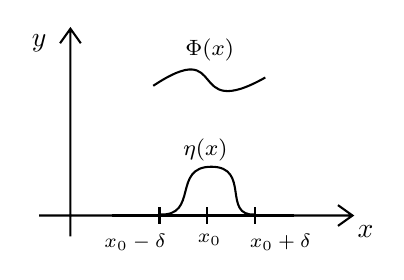
\begin{tikzpicture}[x=0.75pt,y=0.75pt,yscale=-1,xscale=1]
		%uncomment if require: \path (0,142); %set diagram left start at 0, and has height of 142
		
		%Shape: Axis 2D [id:dp3130799933389703] 
		\draw  (57,105) -- (208,105)(72.1,15) -- (72.1,115) (201,100) -- (208,105) -- (201,110) (67.1,22) -- (72.1,15) -- (77.1,22)  ;
		%Curve Lines [id:da7888339580314685] 
		\draw    (112,42.5) .. controls (149,18) and (127,60.5) .. (166,38.5) ;
		%Straight Lines [id:da10959352772350273] 
		\draw    (92,105) -- (180,105) (115,101) -- (115,109)(138,101) -- (138,109)(161,101) -- (161,109) ;
		%Curve Lines [id:da8826440966757665] 
		\draw    (115,104.5) .. controls (134,105.5) and (121,81.5) .. (140,81.5) .. controls (159,81.5) and (145,105.5) .. (161,104.5) ;
		
		% Text Node
		\draw (209,108.4) node [anchor=north west][inner sep=0.75pt]    {$x$};
		% Text Node
		\draw (52,16.4) node [anchor=north west][inner sep=0.75pt]    {$y$};
		% Text Node
		\draw (126,18.4) node [anchor=north west][inner sep=0.75pt]  [font=\footnotesize]  {$\Phi ( x)$};
		% Text Node
		\draw (87,112.4) node [anchor=north west][inner sep=0.75pt]  [font=\scriptsize]  {$x_{0} -\delta $};
		% Text Node
		\draw (157,112.4) node [anchor=north west][inner sep=0.75pt]  [font=\scriptsize]  {$x_{0} +\delta $};
		% Text Node
		\draw (132,112.4) node [anchor=north west][inner sep=0.75pt]  [font=\scriptsize]  {$x_{0}$};
		% Text Node
		\draw (125,66.4) node [anchor=north west][inner sep=0.75pt]  [font=\footnotesize]  {$\eta ( x)$};
		
		
	\end{tikzpicture}
	\caption{~}
	\label{l1:fig:6}
\end{figure}
Тогда
	\begin{equation}
		\label{l1:eq:13}
		\int\limits_a^b \Phi(x)\cdot\eta(x)\,\dd{x}=\int\limits_{x_0-\delta}^{x_0+\delta} \Phi(x)\cdot\eta(x)\,\dd{x}>0,
	\end{equation}
	ибо на интервале $(x_0-\delta,x_0+\delta)$ функции $\Phi(x)$ и $\eta(x)$ положительные. В то же время, так как $\eta(x)$ --- допустимое изменение, то по условию леммы выполняется \eqref{l1:eq:12}. Значит, \eqref{l1:eq:13} неверно и причина этого --- предположение о том, что $\exists x_0$ такой, что $\Phi(x_0)\neq0$. Таким образом $\Phi(x)\equiv0$.
\end{proof}

Уравнение
\begin{equation}
	\label{l1:eq:14}
	 F_y-\der{}{x}F_{y'}=0
\end{equation} 
называется уравнением Эйлера--Лагранжа (\eqref{l1:eq:11} было тождеством, так как туда был подставлен минимайзер). Мы должны искать решение уравнения \eqref{l1:eq:14} с условиями $y(x)\in\Cfn[{[a,b]}]{2}, y(a)=y_0, y(b)=y_1$. Такие решения называются экстремалями.

Проведя в \eqref{l1:eq:14} дифференцирование, мы получим обыкновенное дифференциальное уравнение второго порядка 
\begin{equation}
	\label{l1:eq:15}
	 F_y-F_{y'x}-F_{y'y}\cdot y'-F_{y'y'}\cdot y''=0.
\end{equation}
Решение \eqref{l1:eq:15} ищется при условиях $y(a)=y_0,\ y(b)=y_1$, то есть это не задача Коши, когда при $x=a$ задаётся $y(a),\ y'(a)$, а так называемая \emph{краевая задача}, когда заданы условия на искомую функцию на обоих концах отрезка.
\vspace{0.2cm}

{\noindent\centering\begin{tabular}{p{0.47\textwidth}|p{0.47\textwidth}}
	
	Задача Коши.
	{\centering
	\tikzset{every picture/.style={line width=0.75pt}} %set default line width to 0.75pt        
	
	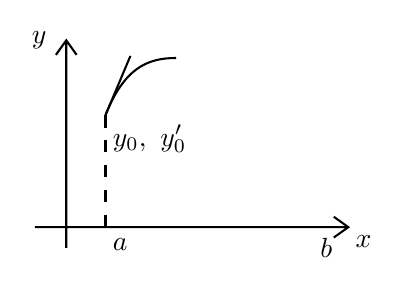
\begin{tikzpicture}[x=0.75pt,y=0.75pt,yscale=-1,xscale=1]
		%uncomment if require: \path (0,142); %set diagram left start at 0, and has height of 142
		
		%Shape: Axis 2D [id:dp5128034111407609] 
		\draw  (57,105) -- (208,105)(72.1,15) -- (72.1,115) (201,100) -- (208,105) -- (201,110) (67.1,22) -- (72.1,15) -- (77.1,22)  ;
		%Curve Lines [id:da7425946058288988] 
		\draw    (91,51) .. controls (100,28.5) and (111,23.5) .. (125,23.5) ;
		%Straight Lines [id:da11481327035855826] 
		\draw  [dash pattern={on 4.5pt off 4.5pt}]  (91,51) -- (91,105.5) ;
		%Straight Lines [id:da16826668588087235] 
		\draw    (91,51) -- (103,22.5) ;
		
		% Text Node
		\draw (93,108.9) node [anchor=north west][inner sep=0.75pt]    {$a$};
		% Text Node
		\draw (193,108.9) node [anchor=north west][inner sep=0.75pt]    {$b$};
		% Text Node
		\draw (210,107.4) node [anchor=north west][inner sep=0.75pt]    {$x$};
		% Text Node
		\draw (54,9.4) node [anchor=north west][inner sep=0.75pt]    {$y$};
		% Text Node
		\draw (93,54.4) node [anchor=north west][inner sep=0.75pt]  [font=\normalsize]  {$y_{0} ,\ y_{0} '$};
		
		
	\end{tikzpicture}

	}
	Задано $y(a)=y_0$, $y'(a)=y_0'$. Другими словами задано значение $y(a)$ и наклон касательной $y'(a)$
	
	& 
	Краевая задача.
	{\centering
	\tikzset{every picture/.style={line width=0.75pt}} %set default line width to 0.75pt        
	
	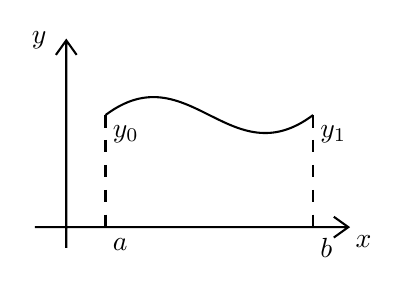
\begin{tikzpicture}[x=0.75pt,y=0.75pt,yscale=-1,xscale=1]
		%uncomment if require: \path (0,142); %set diagram left start at 0, and has height of 142
		
		%Shape: Axis 2D [id:dp6428921470689455] 
		\draw  (57,105) -- (208,105)(72.1,15) -- (72.1,115) (201,100) -- (208,105) -- (201,110) (67.1,22) -- (72.1,15) -- (77.1,22)  ;
		%Curve Lines [id:da5061599430903245] 
		\draw    (91,51) .. controls (131,21) and (151,81) .. (191,51) ;
		%Straight Lines [id:da6222407493262312] 
		\draw  [dash pattern={on 4.5pt off 4.5pt}]  (91,51) -- (91,105.5) ;
		%Straight Lines [id:da8061704415480986] 
		\draw  [dash pattern={on 4.5pt off 4.5pt}]  (191,51) -- (191,105.5) ;
		
		% Text Node
		\draw (93,108.9) node [anchor=north west][inner sep=0.75pt]    {$a$};
		% Text Node
		\draw (193,108.9) node [anchor=north west][inner sep=0.75pt]    {$b$};
		% Text Node
		\draw (210,107.4) node [anchor=north west][inner sep=0.75pt]    {$x$};
		% Text Node
		\draw (54,9.4) node [anchor=north west][inner sep=0.75pt]    {$y$};
		% Text Node
		\draw (93,54.4) node [anchor=north west][inner sep=0.75pt]    {$y_{0}$};
		% Text Node
		\draw (193,54.4) node [anchor=north west][inner sep=0.75pt]    {$y_{1}$};
		
		
	\end{tikzpicture}

	}
	Задано $y(a)=y_0$, $y(b)=y_1$. $y'(a)$~--- не задано, но должно быть таким, чтобы решение \eqref{l1:eq:15} в точке $b$ имело значение $y_1$. 
	\\
	
\end{tabular}
\vspace{0.2cm}

}
Мы уже говорили, что когда минимайзер существует, то, решая \eqref{l1:eq:15}, мы его найдём. Если решений у \eqref{l1:eq:15} нет, то минимайзер --- отсутствует. А теперь главный вопрос: нашли экстремаль (решение \eqref{l1:eq:15}) с заданными граничными условиями: это минимайзер? А может быть это максимайзер (ведь для максимайзера уравнение такое же)? Начнём с того, что найденная экстремаль не обязана быть ни минимайзером, ни максимайзером. Это связанно с тем, что 
\begin{enumerate1}
	\item \label{l1:enum1} Мы сравнивали значение функционала на минимайзере $\J[y]$ не со значением на любой другой функции из $\mc{K}$, а только со значением $\J[y+t\cdot\eta]$ на функциях $y+t\cdot\eta$. Поэтому даже если $y$ --- минимайзер среди этих функций, он может не быть минимайзером во всём классе $\mc{K}$.
	\item \label{l1:enum2} Мы используем \emph{необходимое условие экстремума} --- равенство нулю первой производной, а не достаточное.
\end{enumerate1}

\noindent Обсудим \ref{l1:enum2}. Достаточное условие минимума (среди функций $y+t\?\cdot\eta$\,!)~--- неравенство
\begin{equation*}
	\left.\dder{}{t}\J[y+t\cdot\eta]\right|_{t=0}>0,\quad\forall\eta.
\end{equation*}  
Если оно выполнено, то экстремаль $y(x)$ не может быть максимайзером в $\mc{K}$, иначе она была бы максимайзером среди функций $y+t\cdot\eta$ и тогда
\begin{equation*}
	\left.\dder{}{t}\J[y+t\cdot\eta]\right|_{t=0}<0,
\end{equation*}
а у нас противоположное неравенство. Таким образом, неравенство 
\begin{equation*}
	\left.\dder{}{t}\J[y+t\cdot\eta]\right|_{t=0}>0,\quad\forall\eta
\end{equation*}
говорит, что $y$ не может быть максимайзером (противоположное неравенство запрещает экстремали быть минимайзером).

Из тех же соображений, если знак $\left.\dder{}{t}\J[y+t\cdot\eta]\right|_{t=0}$ зависит от $\eta$,  $y$ не может быть ни минимайзером, ни максимайзером. Это соответствует точке перегиба.   

Что касается \ref{l1:enum1}, то достаточное условие для того, чтобы экстремаль $y(x)$ была минимайзером \{максимайзером\} есть выполнение для всех $\eta$ и какой-либо константы $c_0>0$ неравенства
\begin{equation*}
	\left.\dder{}{t}\J[y+t\cdot\eta]\right|_{t=0}\geqslant c_0\int\limits_a^b\left(\eta^2+\eta^{\prime 2}\right)\,\dd{x},
\end{equation*}
\begin{equation*}
	\left\{\left.\dder{}{t}\J[y+t\cdot\eta]\right|_{t=0}\leqslant -c_0\int\limits_a^b\left(\eta^2+\eta^{\prime 2}\right)\,\dd{x}\right\}.
\end{equation*} 
Причём минимайзер или максимайзер  не во всём классе $\mc{K}$, а среди функций близких к $y$ в метрике
\begin{equation*}
	\sup\limits_{x\in{[a,b]}}\{|y(x)-\hat{y}(x)|+|y'(x)-\hat{y}'(x)|\}<\varepsilon,
\end{equation*} 
где $\varepsilon>0$ --- малое фиксированное число.

Прежде чем переходить к примерам решения уравнения Эйлера, остановимся на важном случае, когда интегрант $F(x,y,y')$ может иметь особенности. Например, в задаче о брахистохроне в знаменателе интегранта содержится $\sqrt{y_0-y(x)}$, и при $x=a$ мы имеем в знаменателе $\sqrt{y_0-y_0}=0$. Выясним, как быть в подобной ситуации. Пусть $[\alpha,\beta]\subset[a,b]$, и на отрезке $[\alpha,\beta]$ функция $F(x,y,y')$ не имеет особенностей. Возьмём допустимое изменение $\eta(x)\equiv0$ вне $[\alpha,\beta]$. Тогда 
\begin{multline*}
	\J[y+t\cdot\eta]=\int\limits_a^b F(x,y+t\cdot\eta,y'+t\cdot\eta')\,\dd{x}=\\=\int\limits_a^\alpha F(x,y,y')\,\dd{x}+\int\limits_{\beta}^b F(x,y,y')\,\dd{x}+\int\limits_{\alpha}^{\beta} F(x,y+t\cdot\eta,y'+t\cdot\eta')\,\dd{x}.
\end{multline*} 
Два первых слагаемых не зависят от $t$. Поэтому
\begin{equation*}
	\der{\J}{t}[y+t\cdot\eta]=\der{}{t}\int\limits_{\alpha}^{\beta} F(x,y+t\cdot\eta,y'+t\cdot\eta')\,\dd{x},
\end{equation*} 
и так как на отрезке $[\alpha,\beta]$ $F\in\Cfn[]{2}$, то мы можем провести все те же рассуждения, что проводили раньше для отрезка $[a,b]$ и получить, что на отрезке $[\alpha,\beta]$
\begin{equation*}
	F_y-\der{}{x}F_{y'}=0.
\end{equation*} 
Отсюда следует, что уравнение Эйлера выполняется в любой точке, где нет особенностей $F$. 

Ещё одно замечание. Мы в классе $\mc{K}$ требуем, чтобы $y\in\Cfn[{[a,b]}]{1}$. Можно заменить его на требование кусочно--непрерывной дифференцируемости, но разрывы производных должны быть типа <<конечного скачка>>. 

В заключение пример задачи, где минимайзер не существует. Пусть
\begin{equation*}
	\J[y]=\int\limits_0^1 x^2\cdot y^{\prime 2}\,\dd{x},\quad \mc{K}=\left\{y(x)\middle|y\in\Cfn[{[0,1]}]{1}, y(0)=1, y(1)=0\right\}.
\end{equation*}
Ясно, что $\J[y]>0, y\in\mc{K}$. Покажем, что $\inf\limits_{y\in\mc{K}}\,\J[y]=0$. Рассмотрим функции 
\begin{equation*}
	y_{\alpha}(x)=
	\begin{cases}
		(x-\alpha)^2 \cdot \frac{1}{\alpha^2}, & 0\leqslant x \leqslant \alpha;\\
		0, & \alpha \leqslant x \leqslant 1;
	\end{cases}
\end{equation*}
где $\alpha>0$ --- малое число.
\begin{figure}[H]\centering
\tikzset{every picture/.style={line width=0.75pt}} %set default line width to 0.75pt        

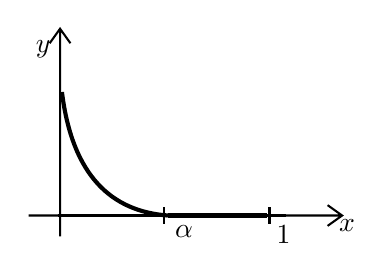
\begin{tikzpicture}[x=0.75pt,y=0.75pt,yscale=-1,xscale=1]
	%uncomment if require: \path (0,142); %set diagram left start at 0, and has height of 142
	
	%Shape: Axis 2D [id:dp09074124062706446] 
	\draw  (57,105) -- (208,105)(72.1,15) -- (72.1,115) (201,100) -- (208,105) -- (201,110) (67.1,22) -- (72.1,15) -- (77.1,22)  ;
	%Curve Lines [id:da6265352586438313] 
	\draw [line width=1.5]    (73,45.5) .. controls (78,86) and (97,103) .. (124,105) ;
	%Straight Lines [id:da7731691289679754] 
	\draw    (71,105) -- (181,105) (122,101) -- (122,109)(173,101) -- (173,109) ;
	%Straight Lines [id:da9057637604000548] 
	\draw [line width=1.5]    (124,105) -- (172,105) ;
	
	% Text Node
	\draw (126,108.4) node [anchor=north west][inner sep=0.75pt]    {$\alpha $};
	% Text Node
	\draw (175,108.4) node [anchor=north west][inner sep=0.75pt]    {$1$};
	% Text Node
	\draw (205,105.4) node [anchor=north west][inner sep=0.75pt]    {$x$};
	% Text Node
	\draw (59,19.4) node [anchor=north west][inner sep=0.75pt]    {$y$};
	
	
\end{tikzpicture}
\caption{~}
\label{l1:fig:7}
\end{figure}
\begin{multline*}
	\J[y_{\alpha}]=4\int\limits_0^{\alpha} x^2\cdot\frac{(x-\alpha)^2}{\alpha^4}\,\dd{x}\leqslant\frac4{\alpha^2}\int\limits_0^{\alpha} (x-\alpha)^2\,\dd{x}=\\=\frac4{3\cdot\alpha^2}(x-\alpha)^3\mathop{\Big|}\limits_0^{\alpha}\to0\text{ при }\alpha\to0.
\end{multline*}  
Значит $\inf\limits_{y\in\mc{K}}\,\J[y]=0$, и поэтому минимайзер не существует.
\vspace{0.2cm}

\noindent\textbf{Задание.} Докажите, что максимайзер тоже не существует.